\begin{savequote}[8cm]
Alice: "How long is forever?" \\
White Rabbit: "Sometimes, just one second."

  \qauthor{--- Lewis Carroll \cite{carroll_alice_1865}}
\end{savequote}

\chapter{Search for Quantum Decoherence in the \texorpdfstring{\acrshort{t2k}}{TEXT} and \texorpdfstring{\acrshort{dune}}{TEXT} Experiments}
%
\minitoc
%
%
\begin{equation} \label{eq:llh}
\begin{aligned}
-\ln(\mathcal{L}) =\;&
\sum_{i}^{\text{NDbins}} 
\left[
N_i^{\text{ND,MC}}(\vec{\theta}) - N_i^{\text{ND,D}} 
+ N_i^{\text{ND,D}} \ln\left(
\frac{N_i^{\text{ND,D}}}{N_i^{\text{ND,MC}}(\vec{\theta})}
\right)
\right]
+ \frac{(\beta_i - 1)^2}{2\sigma_{\beta_i}^2}
\\[0.4em]
&+
\sum_{i}^{\text{FDbins}} 
\left[
N_i^{\text{FD,MC}}(\vec{\theta}) - N_i^{\text{FD,D}} 
+ N_i^{\text{FD,D}} \ln\left(
\frac{N_i^{\text{FD,D}}}{N_i^{\text{FD,MC}}(\vec{\theta})}
\right)
\right]
\\[0.4em]
&+
\sum_{i}^{\text{AtmBins}} 
\left[
N_i^{\text{Atm,MC}}(\vec{\theta}) - N_i^{\text{Atm,D}} 
+ N_i^{\text{Atm,D}} \ln\left(
\frac{N_i^{\text{Atm,D}}}{N_i^{\text{Atm,MC}}(\vec{\theta})}
\right)
\right]
\\[0.4em]
&+
\frac{1}{2}
\sum_{k}
\sum_{i}^{N_b^{(k)}}
\sum_{j}^{N_b^{(k)}}
(\theta_i^{k}) \,(V^{k})^{-1}_{ij}\, (\theta_j^{k}) \,.
\end{aligned}
\end{equation}
%

%
    \begin{figure}[hpbt]
	\centering
	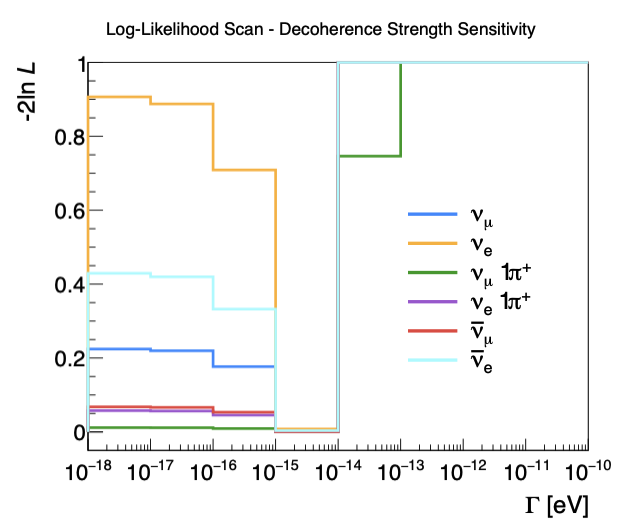
\includegraphics[width=1.\textwidth]{figures/llhscan_t2k_n-2.png}%
	\caption{....}
	\label{fig:llhscan_t2k_n-2}
    \end{figure}
%

\section{Reweighting to Include Experimental Data From Neutrino Reactor Experiments}
In order to include experimental data from neutrino reactor experiments, the posterior can be modified by changing the prior after the posterior has come to its final shape by swapping out the old prior $P_\text{old}(\boldsymbol{\theta})$ for a new prior $P_\text{new}(\boldsymbol{\theta})$, which can be seen by considering an old and a new posterior:
%
\begin{equation} \label{eq:old_new_posterior}
    \begin{aligned}
        P_\text{new}(\boldsymbol{\theta}|\boldsymbol{x}) &=  \mathcal{L}(\boldsymbol{x}|\boldsymbol{\theta}) \cdot P_\text{new}(\boldsymbol{\theta}) \\
        P_\text{new}(\boldsymbol{\theta}|\boldsymbol{x})  &= \mathcal{L}(\boldsymbol{x}|\boldsymbol{\theta}) \cdot P_\text{new}(\boldsymbol{\theta})
        \ \text{.}
    \end{aligned}
\end{equation}  
%
Dividing both equations in \Cref{eq:old_new_posterior} yields the weight that inherits a new constraint on the posterior:
%
\begin{equation} \label{eq:reweight_posterior_weight}
 w_\text{constraint} = \frac{P_\text{new}(\boldsymbol{\theta})}{P_\text{old}(\boldsymbol{\theta})}
 \ \text{,}
 %P(\boldsymbol{\theta}|D) = P(D|\boldsymbol{\theta}) \cdot P(\boldsymbol{\theta}) \ ,
\end{equation}  
%
The weight in \Cref{eq:reweight_posterior_weight} can then be used to evaluate the alternate (unnormalised) posterior from the old one in \Cref{eq:unnormalised_posterior}:
%
\begin{equation} \label{eq:unnormalised_posterior_reweighted}
 P_\text{new}(\boldsymbol{\theta}|\boldsymbol{x}) = P_\text{old}(\boldsymbol{\theta}|\boldsymbol{x}) \cdot w_\text{constraint}
 \ \text{.}
 %P(\boldsymbol{\theta}|D) = P(D|\boldsymbol{\theta}) \cdot P(\boldsymbol{\theta}) \ ,
\end{equation}  
%
In practice, reweighting the posteriors using a Gaussian as new prior $P_\text{new}(\boldsymbol{\theta})$ from the old flat prior $P_\text{old}(\boldsymbol{\theta})$ means to multiply the generated posterior distributions $P_\text{new}(\boldsymbol{\theta}|\boldsymbol{x})$ by
%
\begin{equation} \label{eq:unnormalised_posterior_reweighted}
 w_\text{RC} 
 =
 \frac{P_\text{new}(\boldsymbol{\theta})}{P_\text{old}(\boldsymbol{\theta})}
 = \frac{\text{e}^{-\frac{1}{2} \frac{(\theta - \mu)^2}{\sigma^2}}}{1}
 \ \text{.}
\end{equation}  
%
In case of applying the reactor constraint from measurements by neutrino reactor experiments to the posteriors, $\theta = \sin^2_{13}(\theta)$ with a central value of $0.0219 \pm 0.0007$ \cite{PDG here}.

\chapter{Quantum Decoherence Neutrino Oscillation Analysis} \label{sec:results}
%
\minitoc
%

\section{Sensitivity Studies}
\subsection{T2K A without Reactor Constraints}
\Cref{fig:qd_decostrength_triangleplot_T2K_A2_nh_woRC} shows the one- and two-dimensional posterior distributions for $\Gamma = 0$.
%
    \begin{figure}[hbt]
	\centering
	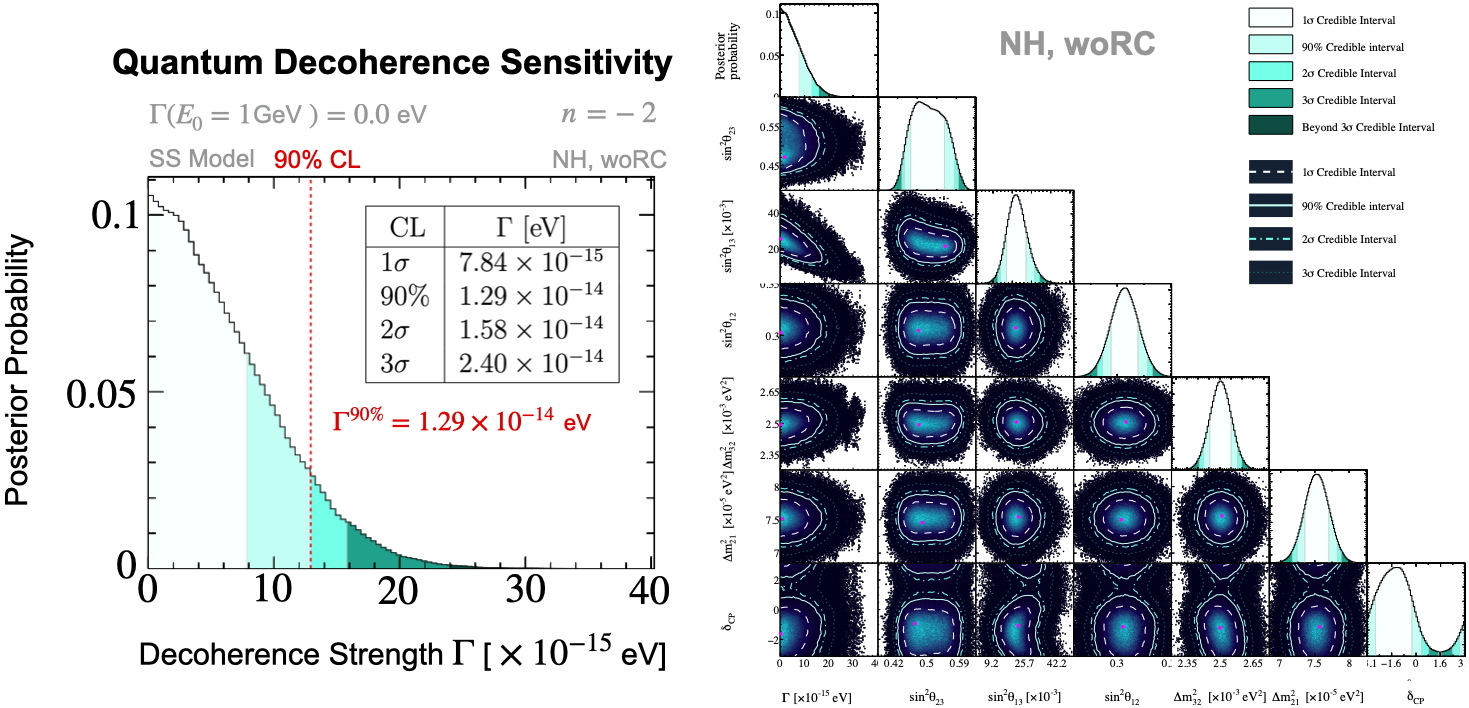
\includegraphics[width=1.\textwidth]{figures/QD_results/qd_decostrength_triangleplot_T2K_A2_nh_woRC.png}
	\caption[T2K A2 nh WoRC.]{T2K A2 nh WoRC.}
	\label{fig:qd_decostrength_triangleplot_T2K_A2_nh_woRC}
    \end{figure}
%
There is an anti-correlation between the decoherence strength $\Gamma$ and the atmospheric mixing angle $\sin^2(\theta_{13})$. This anti-correlation can be understood by looking at the neutrino event rates in dependence on the choice of these two parameters, which is shown in \Cref{fig:anti-corelation_evtrate}. Starting at point $(\Gamma, \sin^2(\theta_{13}) = (\SI{0.0}{\eV}, 0.018)$, the event rate can be increased by raising the decoherence strength to $(\Gamma, \sin^2(\theta_{13}) = (1.29 \times 10^{-14}\ \text{eV}, 0.018)$. The event rate can also be increased by increasing $\sin^2(\theta_{13}$ to $(\Gamma, \sin^2(\theta_{13}) = (1.29 \times 10^{-14}\ \text{eV}, 0.022)$. Then, lowering the decoherence down to $(\Gamma, \sin^2(\theta_{13}) = (\SI{0.0}{\eV}, 0.022)$ yields a comparable event total event rate to the one at $(\Gamma, \sin^2(\theta_{13}) = (1.29 \times 10^{-14}\ \text{eV}, 0.018)$ in $\Gamma$ vs. $\sin^2(\theta_{13}$ parameter space, hence showing the their anti-correlation.
%
    \begin{figure}[hbt]
	\centering
	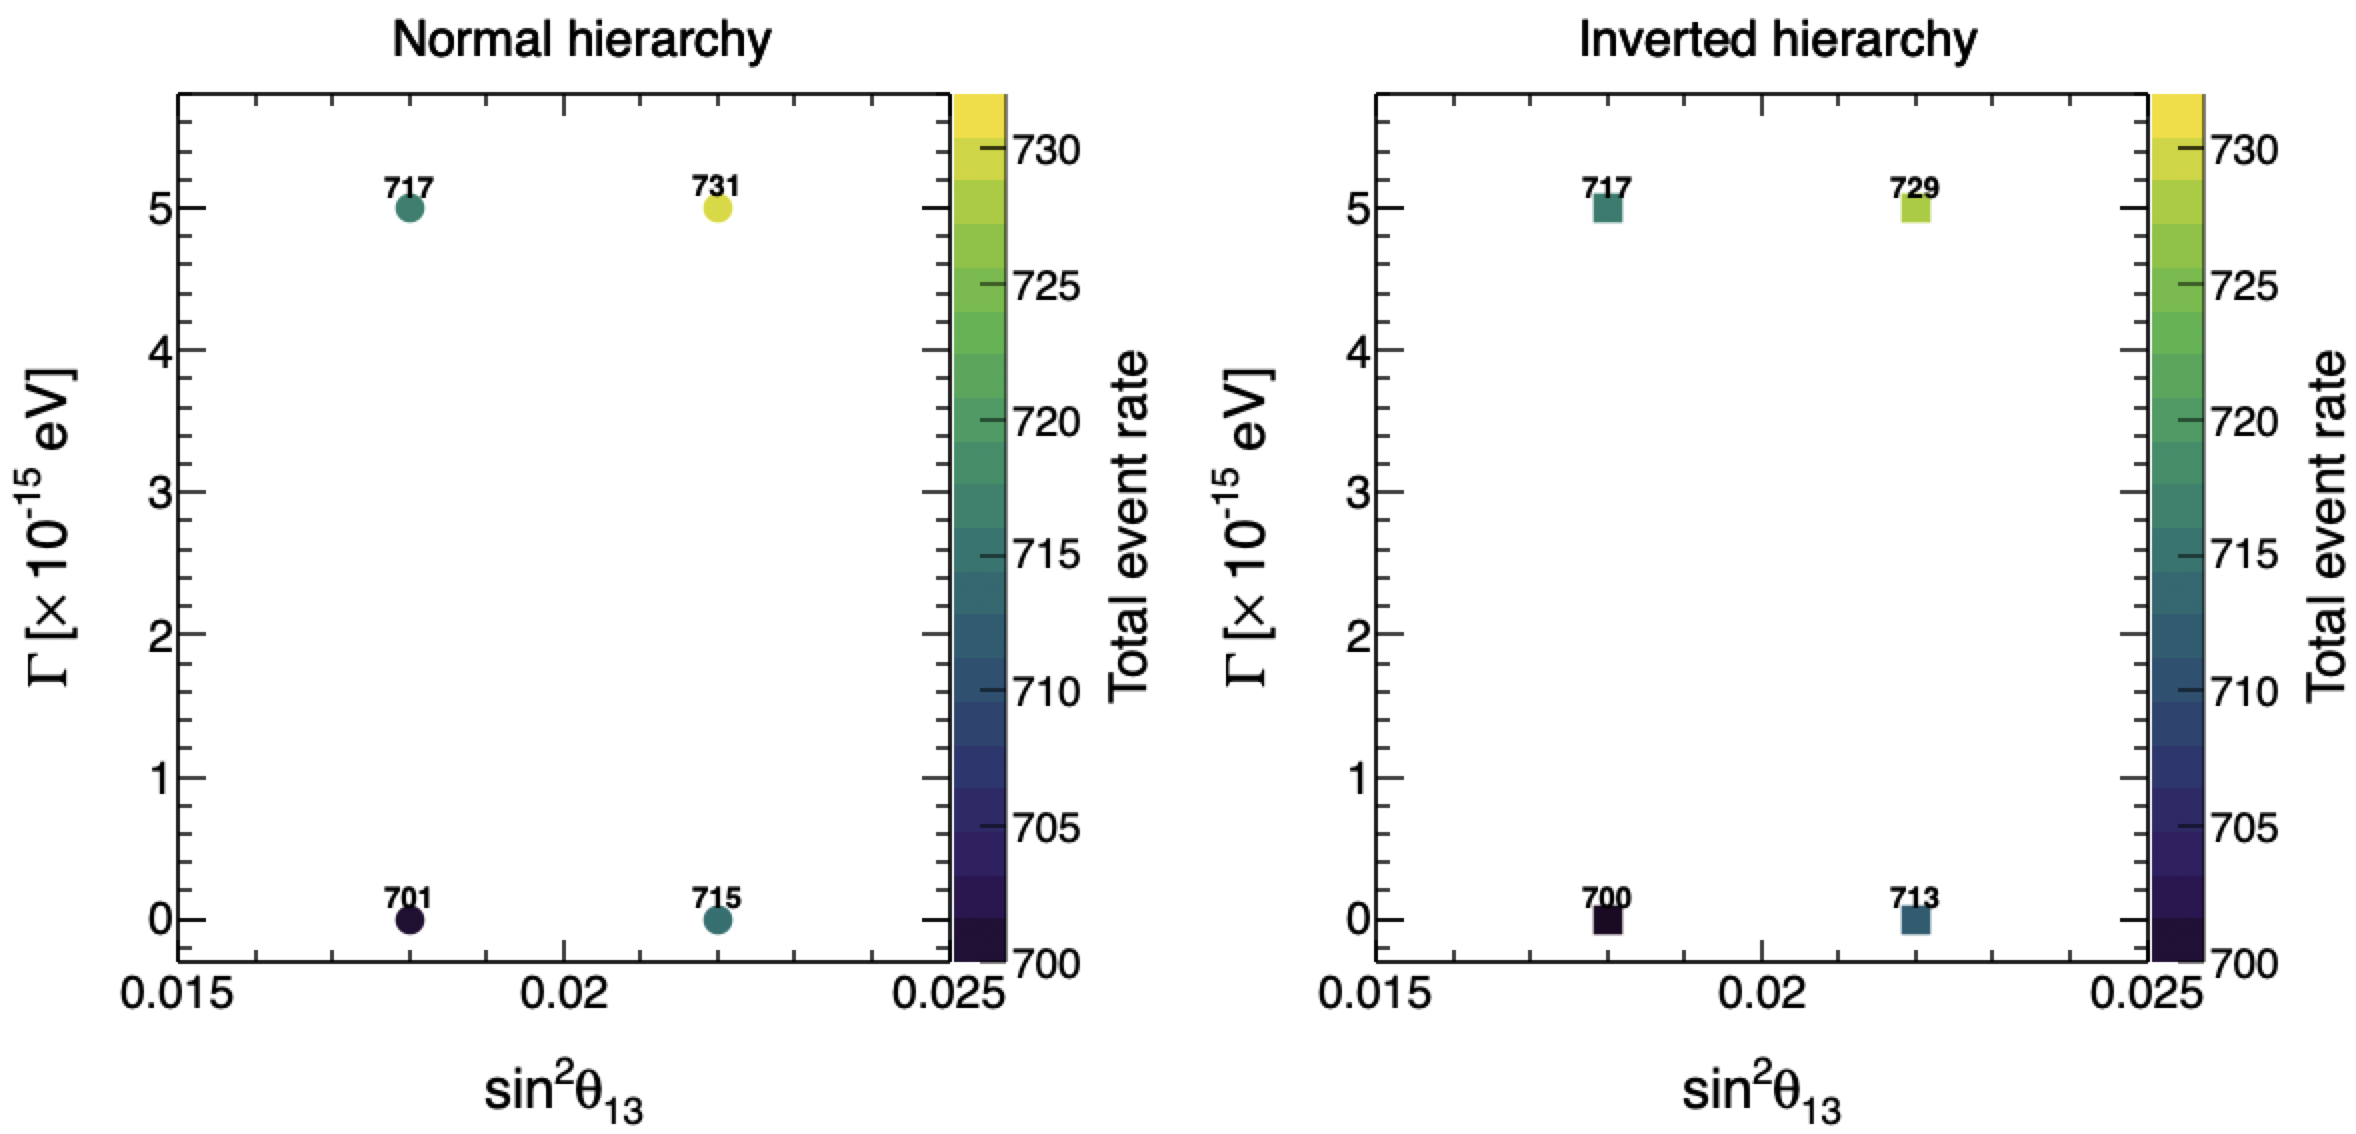
\includegraphics[width=1.\textwidth]{figures/anti-corelation_evtrate.png}
	\caption{anti-corelation-evtrate.}
	\label{fig:anti-corelation_evtrate}
    \end{figure}
%
The $90\%$ credible region goes up to $\Gamma^{90\%} = 1.29 \times 10^{-14} \ \text{eV}$. Explain Marginalisation effect... Turning on reactor constraints means to have less possibilities of raising the event rate by the same amount compared to two variable parameters, so that the $1$-dimensional decoherence strength posterior shifts to higher decoherence strength values and the $90$\% credible region boundary goes down to $\Gamma^{90\%} = 1.12 \times 10^{-14} \ \text{eV}$ compared to the case without reactor constraints.
%
    \begin{figure}[hbt]
	\centering
	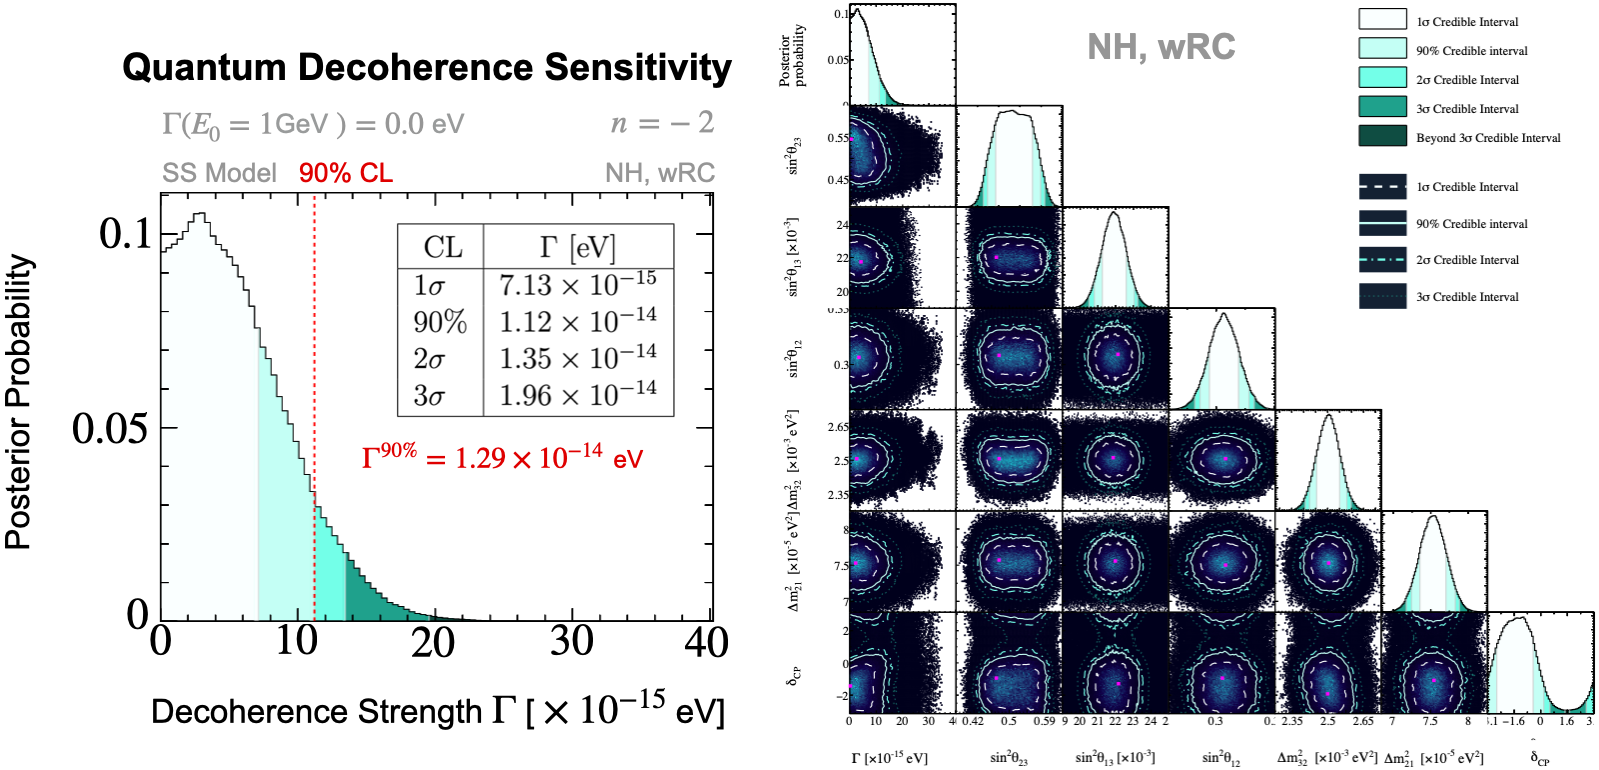
\includegraphics[width=1.\textwidth]{figures/QD_results/qd_decostrength_triangleplot_T2K_A2_nh_wRC.png}
	\caption[T2K A2 nh wRC.]{T2K A2 nh WoRC.}
	\label{fig:qd_decostrength_triangleplot_T2K_A2_nh_wRC}
    \end{figure}
%
B with deco zero, dcp minimal reduces the number of nues, such that decostrength can stay low. this confirms the marginalisation effect seen in \Cref{fig:qd_decostrength_triangleplot_T2K_A2_nh_woRC}. The shifted one-dimensional posterior to lower values of decostrength can be explained by the biprobability plot in \Cref{fig:biprob}.
%
    \begin{figure}[hbt]
	\centering
	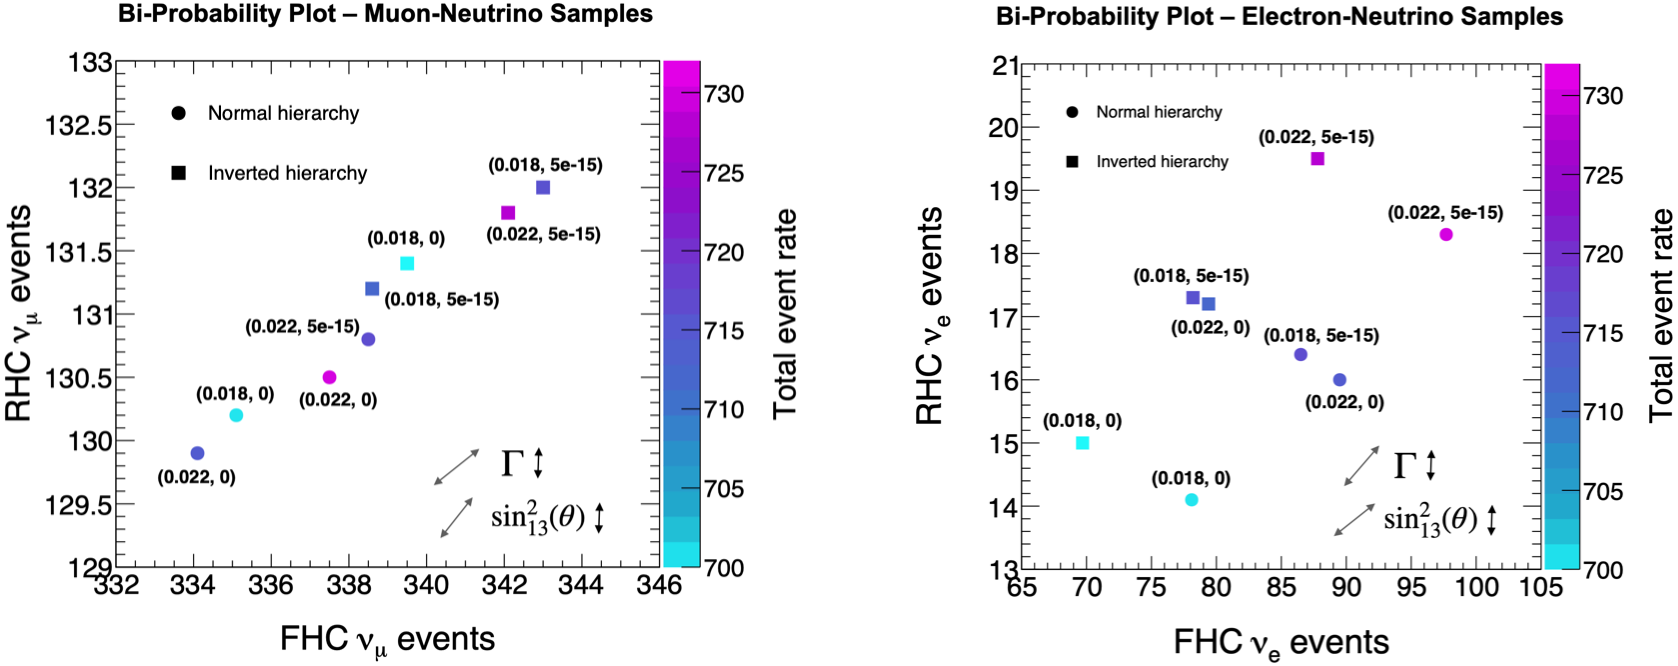
\includegraphics[width=1.\textwidth]{figures/QD_results/biprob.png}
	\caption[biprob.]{biprob.}
	\label{fig:biprob}
    \end{figure}
%
The biprobability plot in \Cref{fig:biprob} shows that if you have your Asimov point in NH and force the fit to be IH, your equivalent oscillation parameters will predict too few electron neutrinos $\nu_\text{e}$ and too many anti-electron neutrinos $\bar{\nu}_\text{e}$. Since the difference in the total event rate in the number of $\nu_\text{e}$ is bigger than the one in $\bar{\nu}_\text{e}$, the $\nu_\text{e}$ have a greater impact to fix the fit. To get more $\nu_\text{e}$ either increase gamma or increase th13 have to be increased. If we restrict th13 (for example with the reactor constraint) then the only option is to increase gamma.

The following results show the effect of decoherence on the oscillation probabilities %{\color{red} Should I show some oscillation probability plots here as well that match the event rate predictions?}
and hence the observed event rates in \acrshort{dune} and \acrshort{t2k}. In \acrshort{dune}, there are four inclusive samples, the \acrshort{cc}$\nu_\mu$, \acrshort{cc}$\bar{\nu}_\mu$, \acrshort{cc}$\nu_e$ and the \acrshort{cc}$\bar{\nu}_e$ samples. In \acrshort{t2k}, there are four exclusive samples, the $\nu_\mu$\acrshort{cc}$0\pi$, $\bar{\nu}_\mu$\acrshort{cc}$0\pi$, $\nu_e$\acrshort{cc}$0\pi$ and the $\bar{\nu}_e$\acrshort{cc}$0\pi$ samples and additional $\nu_\mu$\acrshort{cc}$1\pi^+$ and $\nu_e$\acrshort{cc}$1\pi^+$ samples, so six samples in total. In all plots shown, the reference energy has been set to $E_0 = 1$ GeV. Note, that the choice of $E_0$ does not change the physics but the strength of the decoherence parameter $\Gamma$ to see the same effect. This is demonstrated in \Cref{fig:reference_energy_demo} in which different choices of $\Gamma(E_0)$ and $E_0$ lead to the same decoherence effect on the oscillation probability.
%
    \begin{figure}[hbt]
	\centering
	\includegraphics[width=1.\textwidth]%{Images/Metropolis_Hastings_algorithm_chart.pdf}
    {figures/reference_energy_demo2.pdf}%{Images/reference_energy_demo.pdf}
	\caption{Demonstration of the unphysical change of a different reference energy (left) $E_0=1$ GeV and (right) $E_0=1$ MeV. Dependent on the choice of $E_0$, the decoherence strength $\Gamma(E_0)$ is shifted by a factor of $\left(\frac{E_{0(old)}}{E_{0(new)}}\right)^n$.}
	\label{fig:reference_energy_demo}
    \end{figure}

\subsection{T2K Set A Event Rates}
%
\begin{table}[htbp]
\centering
%\small
\caption{Total number of predicted unoscillated events in Super-Kamiokande for all samples (R$\mu^-$, Re$^-$, R$\mu^-$R$\pi^+$, Re$^-$R$\pi^+$, R$\mu^+$, Re$^+$) for T2K Set A, as a split into interaction channels. $\Gamma 
\neq 0$ means a decoherence strength of $\Gamma = 5.0\times10^{-15}$ eV. The reported data is rounded to one decimal place.}
\resizebox{\textwidth}{!}{
\begin{tabular}{lcccccccccccc}
\toprule
 & \multicolumn{12}{c}{Unoscillated Predicted Events} \\
\cmidrule(lr){2-13}
\multirow{2}{*}{\shortstack{Interaction\\[2pt]Channel}}
& \multicolumn{2}{c}{R$\mu^-$} 
& \multicolumn{2}{c}{Re$^-$} 
& \multicolumn{2}{c}{R$\mu^-$R$\pi^+$}
& \multicolumn{2}{c}{Re$^-$R$\pi^+$}
& \multicolumn{2}{c}{R$\mu^+$}
& \multicolumn{2}{c}{Re$^+$} \\
\cmidrule(lr){2-3} \cmidrule(lr){4-5} \cmidrule(lr){6-7} 
\cmidrule(lr){8-9} \cmidrule(lr){10-11} \cmidrule(lr){12-13}
 & $\Gamma = 0$ & $\Gamma \neq 0$ 
 & $\Gamma = 0$ & $\Gamma \neq 0$ 
 & $\Gamma = 0$ & $\Gamma \neq 0$
 & $\Gamma = 0$ & $\Gamma \neq 0$
 & $\Gamma = 0$ & $\Gamma \neq 0$
 & $\Gamma = 0$ & $\Gamma \neq 0$ \\
\midrule
\acrshort{cc}\acrshort{qe}  & 1049.9 & 1036.8 & 9.5  & 17.2 & 20.3 & 20.2 & 0.6 & 0.6 & 309.3 & 305.7 & 3.0 & 5.0 \\
\acrshort{2p2h}             & 156.8  & 155.2  & 1.8  & 2.9  & 3.0  & 3.0  & 0.2 & 0.2 & 46.9  & 46.4  & 0.6 & 0.8 \\
\acrshort{cc} Other         & 165.7  & 164.5  & 2.3  & 3.7  & 235.3& 234.3& 4.3 & 8.9 & 48.6  & 48.3  & 1.0 & 1.2 \\
\acrshort{nc}               & 13.5   & 13.5   & 5.2  & 5.2  & 6.3  & 6.3  & 1.8 & 1.8 & 4.1   & 4.1   & 1.7 & 1.7 \\
Total                       & 1385.7 & 1370.1 & 19.4 & 29.1 & 265.1& 263.8& 10.4& 11.5& 408.7 & 404.5 & 6.2 & 8.7 \\
\bottomrule
\end{tabular}
}
\end{table}
%
%
\begin{table}[htbp]
\centering
%\small
\caption{Total number of predicted oscillated events in Super-Kamiokande for all samples (R$\mu^-$, Re$^-$, R$\mu^-$R$\pi^+$, Re$^-$R$\pi^+$, R$\mu^+$, Re$^+$) for T2K Set A, as a split into interaction channels. $\Gamma 
\neq 0$ means a decoherence strength of $\Gamma = 5.0\times10^{-15}$ eV. The reported data is rounded to one decimal place.}
\resizebox{\textwidth}{!}{
\begin{tabular}{lcccccccccccc}
\toprule
 & \multicolumn{12}{c}{Oscillated Predicted Events} \\
\cmidrule(lr){2-13}
\multirow{2}{*}{\shortstack{Interaction\\[2pt]Channel}}
& \multicolumn{2}{c}{R$\mu^-$} 
& \multicolumn{2}{c}{Re$^-$} 
& \multicolumn{2}{c}{R$\mu^-$R$\pi^+$}
& \multicolumn{2}{c}{Re$^-$R$\pi^+$}
& \multicolumn{2}{c}{R$\mu^+$}
& \multicolumn{2}{c}{Re$^+$} \\
\cmidrule(lr){2-3} \cmidrule(lr){4-5} \cmidrule(lr){6-7} 
\cmidrule(lr){8-9} \cmidrule(lr){10-11} \cmidrule(lr){12-13}
 & $\Gamma = 0$ & $\Gamma \neq 0$ 
 & $\Gamma = 0$ & $\Gamma \neq 0$ 
 & $\Gamma = 0$ & $\Gamma \neq 0$
 & $\Gamma = 0$ & $\Gamma \neq 0$
 & $\Gamma = 0$ & $\Gamma \neq 0$
 & $\Gamma = 0$ & $\Gamma \neq 0$ \\
\midrule
\acrshort{cc}\acrshort{qe}  & 213.4 & 216.2 & 61.6 & 68.2 & 11.2 & 11.2 & 0.2 & 0.3 & 84.7 & 85.1 & 10.1 & 11.9 \\
\acrshort{2p2h}             & 39.8  & 40.2  & 10.5 & 11.3 & 1.8  & 1.8  & 0.1 & 0.1 & 15.5 & 15.6 & 1.8  & 2.0  \\
\acrshort{cc} Other         & 66.1  & 67.6  & 12.1 & 12.9 & 108.7& 108.2& 15.8& 17.4& 25.5 & 25.7 & 2.5  & 2.7  \\
\acrshort{nc}               & 13.5  & 13.5  & 5.2  & 5.2  & 6.3  & 6.3  & 1.8 & 1.8 & 4.1  & 4.1  & 1.7  & 1.7  \\
Total                       & 334.1 & 337.5 & 89.5 & 97.7 & 127.1& 127.4& 18.6& 19.6& 129.9& 130.5& 16.0 & 18.3 \\
\bottomrule
\end{tabular}
}
\end{table}
%


%
\begin{table}[htbp]
\centering
%\small
\caption{Total number of predicted unoscillated events in Super-Kamiokande for all samples (R$\mu^-$, Re$^-$, R$\mu^-$R$\pi^+$, Re$^-$R$\pi^+$, R$\mu^+$, Re$^+$) for T2K Set A, as a split into oscillation channels. $\Gamma 
\neq 0$ means a decoherence strength of $\Gamma = 5.0\times10^{-15}$ eV. The reported data is rounded to one decimal place.}
\resizebox{\textwidth}{!}{
\begin{tabular}{lcccccccccccc}
\toprule
 & \multicolumn{12}{c}{Unoscillated Predicted Events} \\
\cmidrule(lr){2-13}
\multirow{2}{*}{\shortstack{Oscillation\\[2pt]Channel}}
& \multicolumn{2}{c}{R$\mu^-$} 
& \multicolumn{2}{c}{Re$^-$} 
& \multicolumn{2}{c}{R$\mu^-$R$\pi^+$}
& \multicolumn{2}{c}{Re$^-$R$\pi^+$}
& \multicolumn{2}{c}{R$\mu^+$}
& \multicolumn{2}{c}{Re$^+$} \\
\cmidrule(lr){2-3} \cmidrule(lr){4-5} \cmidrule(lr){6-7} 
\cmidrule(lr){8-9} \cmidrule(lr){10-11} \cmidrule(lr){12-13}
 & $\Gamma = 0$ & $\Gamma \neq 0$ 
 & $\Gamma = 0$ & $\Gamma \neq 0$ 
 & $\Gamma = 0$ & $\Gamma \neq 0$
 & $\Gamma = 0$ & $\Gamma \neq 0$
 & $\Gamma = 0$ & $\Gamma \neq 0$
 & $\Gamma = 0$ & $\Gamma \neq 0$ \\
\midrule
$\nu_\mu \rightarrow \nu_\mu$  
& 1342.8 & 1327.4 & 6.9 & 6.9 & 258.0 & 256.7 & 7.7 & 7.6 & 101.6 & 101.0 & 0.9 & 0.9 \\

$\nu_\text{e} \rightarrow \nu_\text{e}$  
& 0.4 & 0.4 & 11.7 & 11.5 & 0.3 & 0.3 & 2.4 & 2.4 & 0.1 & 0.1 & 1.6 & 1.6 \\

$\bar{\nu}_\mu \rightarrow \bar{\nu}_\mu$  
& 42.5 & 42.2 & 0.3 & 0.3 & 6.9 & 6.9 & 0.2 & 0.2 & 307.0 & 303.4 & 1.3 & 1.3 \\

$\bar{\nu}_\text{e} \rightarrow \bar{\nu}_\text{e}$  
& 0.0 & 0.0 & 0.6 & 0.6 & 0.0 & 0.0 & 0.0 & 0.0 & 0.1 & 0.1 & 2.4 & 2.4 \\

$\nu_\mu \rightarrow \nu_\text{e}$  
& 0.0 & 0.0 & 0.0 & 9.7 & 0.0 & 0.0 & 0.0 & 1.2 & 0.0 & 0.0 & 0.0 & 0.4 \\

$\bar{\nu}_\mu \rightarrow \bar{\nu}_\text{e}$  
& 0.0 & 0.0 & 0.0 & 0.2 & 0.0 & 0.0 & 0.0 & 0.0 & 0.0 & 0.0 & 0.0 & 2.1 \\

Total  
& 1385.7 & 1370.1 & 19.4 & 29.1 & 265.1 & 263.8 & 10.4 & 11.5 & 408.7 & 404.5 & 6.2 & 8.7 \\
\bottomrule
\end{tabular}
}
\end{table}
%

%
\begin{table}[htbp]
\centering
%\small
\caption{Total number of predicted oscillated events in Super-Kamiokande for all samples (R$\mu^-$, Re$^-$, R$\mu^-$R$\pi^+$, Re$^-$R$\pi^+$, R$\mu^+$, Re$^+$) for T2K Set A, as a split into oscillation channels. $\Gamma 
\neq 0$ means a decoherence strength of $\Gamma = 5.0\times10^{-15}$ eV. The reported data is rounded to one decimal place.}
\resizebox{\textwidth}{!}{
\begin{tabular}{lcccccccccccc}
\toprule
 & \multicolumn{12}{c}{Oscillated Predicted Events} \\
\cmidrule(lr){2-13}
\multirow{2}{*}{\shortstack{Oscillation\\[2pt]Channel}}
& \multicolumn{2}{c}{R$\mu^-$} 
& \multicolumn{2}{c}{Re$^-$} 
& \multicolumn{2}{c}{R$\mu^-$R$\pi^+$}
& \multicolumn{2}{c}{Re$^-$R$\pi^+$}
& \multicolumn{2}{c}{R$\mu^+$}
& \multicolumn{2}{c}{Re$^+$} \\
\cmidrule(lr){2-3} \cmidrule(lr){4-5} \cmidrule(lr){6-7} 
\cmidrule(lr){8-9} \cmidrule(lr){10-11} \cmidrule(lr){12-13}
 & $\Gamma = 0$ & $\Gamma \neq 0$ 
 & $\Gamma = 0$ & $\Gamma \neq 0$ 
 & $\Gamma = 0$ & $\Gamma \neq 0$
 & $\Gamma = 0$ & $\Gamma \neq 0$
 & $\Gamma = 0$ & $\Gamma \neq 0$
 & $\Gamma = 0$ & $\Gamma \neq 0$ \\
\midrule
$\nu_\mu \rightarrow \nu_\mu$  
& 311.5 & 314.9 & 5.3 & 5.3 & 121.6 & 121.9 & 3.5 & 3.5 & 50.6 & 50.6 & 0.8 & 0.8 \\

$\nu_\text{e} \rightarrow \nu_\text{e}$  
& 0.4 & 0.4 & 10.9 & 10.7 & 0.2 & 0.2 & 2.3 & 2.3 & 0.1 & 0.1 & 1.5 & 1.5 \\

$\bar{\nu}_\mu \rightarrow \bar{\nu}_\mu$  
& 22.2 & 22.2 & 0.3 & 0.3 & 5.2 & 5.2 & 0.2 & 0.2 & 79.2 & 79.7 & 1.0 & 1.0 \\

$\bar{\nu}_\text{e} \rightarrow \bar{\nu}_\text{e}$  
& 0.0 & 0.0 & 0.6 & 0.6 & 0.0 & 0.0 & 0.0 & 0.0 & 0.1 & 0.1 & 2.3 & 2.2 \\

$\nu_\mu \rightarrow \nu_\text{e}$  
& 0.1 & 0.1 & 71.9 & 80.1 & 0.1 & 0.1 & 12.6 & 13.6 & 0.0 & 0.0 & 2.8 & 3.1 \\

$\bar{\nu}_\mu \rightarrow \bar{\nu}_\text{e}$  
& 0.0 & 0.0 & 0.6 & 0.7 & 0.0 & 0.0 & 0.0 & 0.0 & 0.0 & 0.0 & 7.7 & 9.7 \\

Total  
& 334.1 & 337.5 & 89.5 & 97.7 & 127.1 & 127.4 & 18.6 & 19.6 & 129.9 & 130.5 & 16.0 & 18.3 \\
\bottomrule
\end{tabular}
}
\end{table}
%












\subsection{T2K Set B Event Rates}

%
\begin{table}[htbp]
\centering
\caption{Total number of predicted unoscillated events in Super-Kamiokande for all samples (R$\mu^-$, Re$^-$, R$\mu^-R\pi^+$, Re$^-R\pi^+$, R$\mu^+$, Re$^+$), split into interaction channels. $\Gamma \neq 0$ corresponds to $\Gamma = 5.0\times10^{-15}$ eV.}
\resizebox{\textwidth}{!}{
\begin{tabular}{lcccccccccccc}
\toprule
 & \multicolumn{12}{c}{Unoscillated Predicted Events} \\
\cmidrule(lr){2-13}
\multirow{2}{*}{Channel}
& \multicolumn{2}{c}{R$\mu^-$} 
& \multicolumn{2}{c}{Re$^-$} 
& \multicolumn{2}{c}{R$\mu^-R\pi^+$}
& \multicolumn{2}{c}{Re$^-R\pi^+$}
& \multicolumn{2}{c}{R$\mu^+$}
& \multicolumn{2}{c}{Re$^+$} \\
\cmidrule(lr){2-13}
 & $\Gamma=0$ & $\neq0$ & $\Gamma=0$ & $\neq0$ & $\Gamma=0$ & $\neq0$
 & $\Gamma=0$ & $\neq0$ & $\Gamma=0$ & $\neq0$ & $\Gamma=0$ & $\neq0$ \\
\midrule
CCQE  & 1049.9 & 1036.8 & 9.5 & 17.2 & 20.3 & 20.2 & 0.6 & 0.6 & 309.3 & 305.7 & 3.0 & 5.0 \\
2p2h  & 156.8  & 155.2  & 1.8 & 2.9  & 3.0  & 3.0  & 0.2 & 0.2 & 46.9  & 46.4  & 0.6 & 0.8 \\
CC other & 165.7 & 164.5 & 2.3 & 3.7 & 235.3 & 234.3 & 4.3 & 8.9 & 48.6 & 48.3 & 1.0 & 1.2 \\
NC    & 13.5   & 13.5   & 5.2 & 5.2  & 6.3  & 6.3  & 1.8 & 1.8 & 4.1   & 4.1   & 1.7 & 1.7 \\
\midrule
Total & 1385.7 & 1370.1 & 19.4 & 29.1 & 265.1 & 263.8 & 10.4 & 11.5 & 408.7 & 404.5 & 6.2 & 8.7 \\
\bottomrule
\end{tabular}
}
\end{table}
%
\begin{table}[htbp]
\centering
%\small
\caption{Total number of predicted oscillated events in Super-Kamiokande for all samples (R$\mu^-$, Re$^-$, R$\mu^-$R$\pi^+$, Re$^-$R$\pi^+$, R$\mu^+$, Re$^+$) for T2K Set B, as a split into interaction channels. $\Gamma 
\neq 0$ means a decoherence strength of $\Gamma = 5.0\times10^{-15}$ eV. The reported data is rounded to one decimal place.}
\resizebox{\textwidth}{!}{
\begin{tabular}{lcccccccccccc}
\toprule
 & \multicolumn{12}{c}{Oscillated Predicted Events} \\
\cmidrule(lr){2-13}
\multirow{2}{*}{\shortstack{Interaction\\[2pt]Channel}}
& \multicolumn{2}{c}{R$\mu^-$} 
& \multicolumn{2}{c}{Re$^-$} 
& \multicolumn{2}{c}{R$\mu^-$R$\pi^+$}
& \multicolumn{2}{c}{Re$^-$R$\pi^+$}
& \multicolumn{2}{c}{R$\mu^+$}
& \multicolumn{2}{c}{Re$^+$} \\
\cmidrule(lr){2-3} \cmidrule(lr){4-5} \cmidrule(lr){6-7} 
\cmidrule(lr){8-9} \cmidrule(lr){10-11} \cmidrule(lr){12-13}
 & $\Gamma = 0$ & $\Gamma \neq 0$ 
 & $\Gamma = 0$ & $\Gamma \neq 0$ 
 & $\Gamma = 0$ & $\Gamma \neq 0$
 & $\Gamma = 0$ & $\Gamma \neq 0$
 & $\Gamma = 0$ & $\Gamma \neq 0$
 & $\Gamma = 0$ & $\Gamma \neq 0$ \\
\midrule
\acrshort{cc}\acrshort{qe}  & 213.4 & 216.2 & 61.6 & 68.2 & 11.2 & 11.2 & 0.2 & 0.3 & 84.7 & 85.1 & 10.1 & 11.9 \\
\acrshort{2p2h}             & 39.8  & 40.2  & 10.5 & 11.3 & 1.8  & 1.8  & 0.1 & 0.1 & 15.5 & 15.6 & 1.8  & 2.0  \\
\acrshort{cc} Other         & 66.1  & 67.6  & 12.1 & 12.9 & 108.7& 108.2& 15.8& 17.4& 25.5 & 25.7 & 2.5  & 2.7  \\
\acrshort{nc}               & 13.5  & 13.5  & 5.2  & 5.2  & 6.3  & 6.3  & 1.8 & 1.8 & 4.1  & 4.1  & 1.7  & 1.7  \\
Total                       & 334.1 & 337.5 & 89.5 & 97.7 & 127.1& 127.4& 18.6& 19.6& 129.9& 130.5& 16.0 & 18.3 \\
\bottomrule
\end{tabular}
}
\end{table}
%


%
\begin{table}[htbp]
\centering
%\small
\caption{Total number of predicted unoscillated events in Super-Kamiokande for all samples (R$\mu^-$, Re$^-$, R$\mu^-$R$\pi^+$, Re$^-$R$\pi^+$, R$\mu^+$, Re$^+$) for T2K Set B, as a split into oscillation channels. $\Gamma 
\neq 0$ means a decoherence strength of $\Gamma = 5.0\times10^{-15}$ eV. The reported data is rounded to one decimal place.}
\resizebox{\textwidth}{!}{
\begin{tabular}{lcccccccccccc}
\toprule
 & \multicolumn{12}{c}{Unoscillated Predicted Events} \\
\cmidrule(lr){2-13}
\multirow{2}{*}{\shortstack{Oscillation\\[2pt]Channel}}
& \multicolumn{2}{c}{R$\mu^-$} 
& \multicolumn{2}{c}{Re$^-$} 
& \multicolumn{2}{c}{R$\mu^-$R$\pi^+$}
& \multicolumn{2}{c}{Re$^-$R$\pi^+$}
& \multicolumn{2}{c}{R$\mu^+$}
& \multicolumn{2}{c}{Re$^+$} \\
\cmidrule(lr){2-3} \cmidrule(lr){4-5} \cmidrule(lr){6-7} 
\cmidrule(lr){8-9} \cmidrule(lr){10-11} \cmidrule(lr){12-13}
 & $\Gamma = 0$ & $\Gamma \neq 0$ 
 & $\Gamma = 0$ & $\Gamma \neq 0$ 
 & $\Gamma = 0$ & $\Gamma \neq 0$
 & $\Gamma = 0$ & $\Gamma \neq 0$
 & $\Gamma = 0$ & $\Gamma \neq 0$
 & $\Gamma = 0$ & $\Gamma \neq 0$ \\
\midrule
$\nu_\mu \rightarrow \nu_\mu$  
& 1342.8 & 1327.4 & 6.9 & 6.9 & 258.0 & 256.7 & 7.7 & 7.6 & 101.6 & 101.0 & 0.9 & 0.9 \\

$\nu_\text{e} \rightarrow \nu_\text{e}$  
& 0.4 & 0.4 & 11.7 & 11.5 & 0.3 & 0.3 & 2.4 & 2.4 & 0.1 & 0.1 & 1.6 & 1.6 \\

$\bar{\nu}_\mu \rightarrow \bar{\nu}_\mu$  
& 42.5 & 42.2 & 0.3 & 0.3 & 6.9 & 6.9 & 0.2 & 0.2 & 307.0 & 303.4 & 1.3 & 1.3 \\

$\bar{\nu}_\text{e} \rightarrow \bar{\nu}_\text{e}$  
& 0.0 & 0.0 & 0.6 & 0.6 & 0.0 & 0.0 & 0.0 & 0.0 & 0.1 & 0.1 & 2.4 & 2.4 \\

$\nu_\mu \rightarrow \nu_\text{e}$  
& 0.0 & 0.0 & 0.0 & 9.7 & 0.0 & 0.0 & 0.0 & 1.2 & 0.0 & 0.0 & 0.0 & 0.4 \\

$\bar{\nu}_\mu \rightarrow \bar{\nu}_\text{e}$  
& 0.0 & 0.0 & 0.0 & 0.2 & 0.0 & 0.0 & 0.0 & 0.0 & 0.0 & 0.0 & 0.0 & 2.1 \\

Total  
& 1385.7 & 1370.1 & 19.4 & 29.1 & 265.1 & 263.8 & 10.4 & 11.5 & 408.7 & 404.5 & 6.2 & 8.7 \\
\bottomrule
\end{tabular}
}
\end{table}
%

%
\begin{table}[htbp]
\centering
%\small
\caption{Total number of predicted oscillated events in Super-Kamiokande for all samples (R$\mu^-$, Re$^-$, R$\mu^-$R$\pi^+$, Re$^-$R$\pi^+$, R$\mu^+$, Re$^+$) for T2K Set B, as a split into oscillation channels. $\Gamma 
\neq 0$ means a decoherence strength of $\Gamma = 5.0\times10^{-15}$ eV. The reported data is rounded to one decimal place.}
\resizebox{\textwidth}{!}{
\begin{tabular}{lcccccccccccc}
\toprule
 & \multicolumn{12}{c}{Oscillated Predicted Events} \\
\cmidrule(lr){2-13}
\multirow{2}{*}{\shortstack{Oscillation\\[2pt]Channel}}
& \multicolumn{2}{c}{R$\mu^-$} 
& \multicolumn{2}{c}{Re$^-$} 
& \multicolumn{2}{c}{R$\mu^-$R$\pi^+$}
& \multicolumn{2}{c}{Re$^-$R$\pi^+$}
& \multicolumn{2}{c}{R$\mu^+$}
& \multicolumn{2}{c}{Re$^+$} \\
\cmidrule(lr){2-3} \cmidrule(lr){4-5} \cmidrule(lr){6-7} 
\cmidrule(lr){8-9} \cmidrule(lr){10-11} \cmidrule(lr){12-13}
 & $\Gamma = 0$ & $\Gamma \neq 0$ 
 & $\Gamma = 0$ & $\Gamma \neq 0$ 
 & $\Gamma = 0$ & $\Gamma \neq 0$
 & $\Gamma = 0$ & $\Gamma \neq 0$
 & $\Gamma = 0$ & $\Gamma \neq 0$
 & $\Gamma = 0$ & $\Gamma \neq 0$ \\
\midrule
$\nu_\mu \rightarrow \nu_\mu$  
& 311.5 & 314.9 & 5.3 & 5.3 & 121.6 & 121.9 & 3.5 & 3.5 & 50.6 & 50.6 & 0.8 & 0.8 \\

$\nu_\text{e} \rightarrow \nu_\text{e}$  
& 0.4 & 0.4 & 10.9 & 10.7 & 0.2 & 0.2 & 2.3 & 2.3 & 0.1 & 0.1 & 1.5 & 1.5 \\

$\bar{\nu}_\mu \rightarrow \bar{\nu}_\mu$  
& 22.2 & 22.2 & 0.3 & 0.3 & 5.2 & 5.2 & 0.2 & 0.2 & 79.2 & 79.7 & 1.0 & 1.0 \\

$\bar{\nu}_\text{e} \rightarrow \bar{\nu}_\text{e}$  
& 0.0 & 0.0 & 0.6 & 0.6 & 0.0 & 0.0 & 0.0 & 0.0 & 0.1 & 0.1 & 2.3 & 2.2 \\

$\nu_\mu \rightarrow \nu_\text{e}$  
& 0.1 & 0.1 & 71.9 & 80.1 & 0.1 & 0.1 & 12.6 & 13.6 & 0.0 & 0.0 & 2.8 & 3.1 \\

$\bar{\nu}_\mu \rightarrow \bar{\nu}_\text{e}$  
& 0.0 & 0.0 & 0.6 & 0.7 & 0.0 & 0.0 & 0.0 & 0.0 & 0.0 & 0.0 & 7.7 & 9.7 \\

Total  
& 334.1 & 337.5 & 89.5 & 97.7 & 127.1 & 127.4 & 18.6 & 19.6 & 129.9 & 130.5 & 16.0 & 18.3 \\
\bottomrule
\end{tabular}
}
\end{table}
%



%
\iffalse
%
\begin{table}[htbp]
\centering
%\small
\caption{Total number of predicted oscillated events in Super-Kamiokande for all samples (R$\mu^-$, Re$^-$, R$\mu^-$R$\pi^+$, Re$^-$R$\pi^+$, R$\mu^+$, Re$^+$), as a split into interaction channels. $\Gamma 
\neq 0$ means a decoherence strength of $\Gamma = 5.0\times10^{-15}$ eV.}
\begin{tabular}{llccccc}
\toprule
$\nu_\mu \rightarrow \nu_\mu$  & 311.5 & 314.9 & 5.3  & 5.3  & 121.6 & 121.9 & 3.5 & 3.5 & 50.6  & 50.6  & 0.8 & 0.8 \\
$\nu_\text{e} \rightarrow \nu_\text{e}$  
                              & 0.4   & 0.4   & 10.9 & 10.7 & 0.2   & 0.2   & 2.3 & 2.3 & 0.1   & 0.1   & 1.5 & 1.5 \\
$\bar{\nu}_\mu \rightarrow \bar{\nu}_\mu$ 
                              & 22.2  & 22.2  & 0.3  & 0.3  & 5.2   & 5.2   & 0.2 & 0.2 & 79.2  & 79.7  & 1.0 & 1.0 \\
$\bar{\nu}_\text{e} \rightarrow \bar{\nu}_\text{e}$ 
                              & 0.0   & 0.0   & 0.6  & 0.6  & 0.0   & 0.0   & 0.0 & 0.0 & 0.1   & 0.1   & 2.3 & 2.3 \\
$\nu_\mu \rightarrow \nu_\text{e}$ 
                              & 0.1   & 0.1   & 71.9 & 80.1 & 0.1   & 0.1   & 13.6& 12.6& 0.0   & 0.0   & 3.1 & 2.8 \\
$\bar{\nu}_\mu \rightarrow \bar{\nu}_\text{e}$ 
                              & 0.0   & 0.0   & 0.6  & 0.7  & 0.0   & 0.0   & 0.0 & 0.0 & 0.0   & 0.0   & 9.6 & 7.7 \\
Total                         & 334.1 & 337.5 & 89.5 & 97.7 & 127.1 & 127.4 & 18.6& 19.6& 129.9 & 130.5 & 16.0& 18.3 \\
\bottomrule
\end{tabular}
\end{table}
%
\fi
%


\subsection{DUNE Event Rates}
%
\begin{table}[htbp]
\centering
%\small
\caption{Total number of predicted unoscillated events in the DUNE far detector complex for all samples ($\nu_\mu$: FHC numu, $\nu_\text{e}$: FHC nue, $\bar{\nu}_\mu$: RHC numu, $\bar{\nu}_\text{e}$: RHC nue), split into oscillation channels. $\Gamma 
\neq 0$ means a decoherence strength of $\Gamma = 1.0\times10^{-15}$ eV. The reported data is rounded to one decimal place.}
\resizebox{\textwidth}{!}{
\begin{tabular}{lcccccccc}
\toprule
 & \multicolumn{8}{c}{Unoscillated Predicted Events} \\
\cmidrule(lr){2-9}
\multirow{2}{*}{\shortstack{Oscillation\\[2pt]Channel}}
& \multicolumn{2}{c}{$\nu_\mu$}
& \multicolumn{2}{c}{$\nu_\text{e}$}
& \multicolumn{2}{c}{$\bar{\nu}_\mu$}
& \multicolumn{2}{c}{$\bar{\nu}_\text{e}$} \\
\cmidrule(lr){2-3} \cmidrule(lr){4-5} \cmidrule(lr){6-7} \cmidrule(lr){8-9}
& $\Gamma = 0$ & $\Gamma \neq 0$
& $\Gamma = 0$ & $\Gamma \neq 0$
& $\Gamma = 0$ & $\Gamma \neq 0$
& $\Gamma = 0$ & $\Gamma \neq 0$ \\
\midrule
$\nu_\mu \rightarrow \nu_\mu$                        & 9662.2 & 9659.7  & 105.1 & 105.1  & 2973.1 & 2963.6  & 28.1  & 28.0  \\
$\nu_\text{e} \rightarrow \nu_\text{e}$             & 9.3    & 9.3     & 284.4 & 283.2  & 4.9    & 4.9     & 122.6 & 122.0 \\
$\bar{\nu}_\mu \rightarrow \bar{\nu}_\mu$           & 873.7  & 871.2   & 7.4   & 7.4    & 3087.0 & 3089.0  & 26.4  & 26.4  \\
$\bar{\nu}_\text{e} \rightarrow \bar{\nu}_\text{e}$ & 1.2    & 1.2     & 49.5  & 49.2   & 1.7    & 1.7     & 101.4 & 101.0 \\
$\nu_\mu \rightarrow \nu_\text{e}$                  & 7.7    & 8.1     & 1319.1& 1362.0 & 1.3    & 1.4     & 93.1  & 98.9  \\
$\bar{\nu}_\mu \rightarrow \bar{\nu}_\text{e}$      & 0.0    & 0.1     & 13.2  & 15.5   & 0.3    & 0.4     & 142.6 & 161.9 \\
$\nu_\text{e} \rightarrow \nu_\mu$                  & 7.4    & 8.2     & 0.0   & 0.0    & 2.2    & 2.6     & 0.0   & 0.0   \\
$\bar{\nu}_\text{e} \rightarrow \bar{\nu}_\mu$      & 0.8    & 0.9     & 0.0   & 0.0    & 2.1    & 2.4     & 0.0   & 0.0   \\
$\nu_\mu \rightarrow \nu_\tau$                      & 55.6   & 56.0    & 35.9  & 36.1   & 20.8   & 21.1    & 13.2  & 13.4  \\
$\nu_\text{e} \rightarrow \nu_\tau$                 & 0.1    & 0.1     & 0.1   & 0.1    & 0.1    & 0.1     & 0.0   & 0.1   \\
$\bar{\nu}_\mu \rightarrow \bar{\nu}_\tau$          & 7.1    & 7.1     & 5.2   & 5.2    & 16.6   & 16.8    & 12.1  & 12.2  \\
$\bar{\nu}_\text{e} \rightarrow \bar{\nu}_\tau$     & 0.0    & 0.0     & 0.0   & 0.0    & 0.0    & 0.0     & 0.0   & 0.0   \\
Total                                               & 10625.1& 10621.8 & 1819.8& 1863.9 & 6110.2 & 6104.0  & 539.5 & 563.8 \\
\bottomrule
\end{tabular}
}
\end{table}
%


%
\begin{table}[htbp]
\centering
%\small
\caption{Total number of predicted oscillated events in the DUNE far detector complex for all samples ($\nu_\mu$: FHC numu, $\nu_\text{e}$: FHC nue, $\bar{\nu}_\mu$: RHC numu, $\bar{\nu}_\text{e}$: RHC nue), split into interaction channels. $\Gamma 
\neq 0$ means a decoherence strength of $\Gamma = 1.0\times10^{-15}$ eV. The reported data is rounded to one decimal place.}
\resizebox{\textwidth}{!}{
\begin{tabular}{lcccccccc}
\toprule
 & \multicolumn{8}{c}{Oscillated Predicted Events} \\
\cmidrule(lr){2-9}
\multirow{2}{*}{\shortstack{Interaction\\[2pt]Channel}}
& \multicolumn{2}{c}{$\nu_\mu$}
& \multicolumn{2}{c}{$\nu_\text{e}$}
& \multicolumn{2}{c}{$\bar{\nu}_\mu$}
& \multicolumn{2}{c}{$\bar{\nu}_\text{e}$} \\
\cmidrule(lr){2-3} \cmidrule(lr){4-5} \cmidrule(lr){6-7} \cmidrule(lr){8-9}
& $\Gamma = 0$ & $\Gamma \neq 0$
& $\Gamma = 0$ & $\Gamma \neq 0$
& $\Gamma = 0$ & $\Gamma \neq 0$
& $\Gamma = 0$ & $\Gamma \neq 0$ \\
\midrule
\acrshort{cc}\acrshort{qe}  & 2149.4 & 2150.1 & 440.8 & 451.8 & 973.6 & 973.8 & 103.8 & 109.4 \\
\acrshort{2p2h}             & 581.9  & 582.1  & 120.6 & 123.8 & 329.8 & 330.0 & 33.3  & 35.4  \\
\acrshort{cc} Other         & 7654.3 & 7650.1 & 1168.6& 1198.5& 4680.3& 4673.7& 356.9 & 373.6 \\
\acrshort{nc}               & 239.5  & 239.5  & 89.9  & 89.9  & 126.5 & 126.5 & 45.5  & 45.5  \\
Total                       & 10625.1& 10621.8& 1819.8& 1863.9& 6110.2& 6104.0& 539.5 & 563.8 \\
\bottomrule
\end{tabular}
}
\end{table}
%


In the Bayesian highest posterior density (HPD) approach, a credible interval from a given posterior is given by
%
\begin{align} \label{eq:hbp}
   \int_0^{x_0} p(x) \text{d}x = 0.90 \quad \text{,}
\end{align}
%
and gives the $90\%$ credible limit.

In the frequentist approach, the $\Delta\chi^2$ Confidence Level upper limit,
%
\begin{align} \label{eq:chi2-limit}
   \Delta\chi^2 = 2.71 \quad \text{,}
\end{align}
%
gives a frequentist-style $90\%$ Confidence Level upper limit.

The two approaches in \cref{eq:hbp} and \cref{eq:chi2-limit} are not the same unless the posterior in \cref{eq:hbp} is Gaussian, which is called the \textit{Bernstein–von Mises theorem}.

\newpage
\begin{landscape}
%
\begin{table}[htb]
	\caption[]{World Leading Upper Limits and Sensititivities of Quantum decoherence parameter $\Gamma_0 \ [\text{eV}]$ for a reference energy $E_0 = 1 \ \text{GeV}$ and different choices for the decoherence model and energy scale $n$. Models - 
    Phase Perturbation \cite{QD_Stutt_Jens_2020} (Case $2$ in \cite{Gomes:2020muc}): $D = \text{diag}(0,\Gamma_0,\Gamma_0,0,\Gamma_0,\Gamma_0,\Gamma_0,\Gamma_0,0)$; 
    State Selected \cite{QD_Stutt_Jens_2020} (Case $1$ in \cite{Gomes:2020muc}): $D = \text{diag}(0,\Gamma_0,\Gamma_0,\Gamma_0,\Gamma_0,\Gamma_0,\Gamma_0,\Gamma_0,\Gamma_0)$; 
    Neutrino Loss \cite{QD_Stutt_Jens_2020}: $D = \text{diag}(\Gamma_0,\Gamma_0,\Gamma_0,\Gamma_0,\Gamma_0,\Gamma_0,\Gamma_0,\Gamma_0,\Gamma_0)$; 
    Entanglement (Entropy) \cite{Abdolalizadeh:2024sxp}:;
    Neutrino Magnetic Moment \cite{Ahluwalia:1996ev,Ahluwalia:1998jx}:;
    A \cite{DeRomeri:2023dht}: $D = \text{diag}(\Gamma_0,\Gamma_0,0,\Gamma_0,\Gamma_0,\Gamma_0,\Gamma_0,\Gamma_0,0)$; 
    B \cite{DeRomeri:2023dht}: $D = \text{diag}(\Gamma_0,\Gamma_0,0,\Gamma_0,\Gamma_0,\Gamma_0,0,0,0)$; 
    C \cite{DeRomeri:2023dht}: $D = \text{diag}(\Gamma_0,\Gamma_0,0,0,0,\Gamma_0,\Gamma_0,\Gamma_0,0)$; 
    D \cite{DeRomeri:2023dht}: $D = \text{diag}(0,0,0,\Gamma_0,\Gamma_0,\Gamma_0,\Gamma_0,\Gamma_0,0)$; 
    E \cite{DeRomeri:2023dht}: $D = \text{diag}(\Gamma_0,\Gamma_0,0,0,0,0,0,0,0)$; 
    F \cite{DeRomeri:2023dht}: $D = \text{diag}(0,0,0,\Gamma_0,\Gamma_0,0,0,0,0)$; 
    G \cite{DeRomeri:2023dht}: $D = \text{diag}(0,0,0,0,0,0,\Gamma_0,\Gamma_0,0)$;
    Case $3$ \cite{Gomes:2020muc}: $D = \text{diag}(0,0,0,0,\Gamma_0,\Gamma_0,\Gamma_0,\Gamma_0,0)$
    . 
    Experiments - Purple: IceCube; Blue: Minos.} \label{tab:decoh_up_sen}
    \resizebox{\textwidth}{!}{%
	\begin{tabular}{|l||c|c|c|c|c|c|c|c|c|} \hline
    \diagbox{\text{Model}}{\text{Energy Scale}} & $n=-3$ & $n=-2$ & $n=-1$ & $n=0$ & $n=1$ & $n=2$ & $n=3$ & n=? \\ \hline \hline
    \text{Phase Perturbation} & & & & \cellcolor{violet!25} $1.18\times10^{-15}$ \cite{ICECUBE:2023gdv} & \cellcolor{violet!25} $6.89\times10^{-19}$ \cite{ICECUBE:2023gdv} & \cellcolor{violet!25} $9.8\times10^{-24}$ \cite{ICECUBE:2023gdv} & \cellcolor{violet!25} $1.58\times10^{-28}$ \cite{ICECUBE:2023gdv} & \\ \hline
    \text{State Selected} & & & & \cellcolor{violet!25} $1.17\times10^{-15}$ \cite{ICECUBE:2023gdv} & \cellcolor{violet!25} $6.67\times10^{-19}$ \cite{ICECUBE:2023gdv} & \cellcolor{violet!25} $9.48\times10^{-24}$ \cite{ICECUBE:2023gdv} & \cellcolor{violet!25} $1.17\times10^{-28}$ \cite{ICECUBE:2023gdv} & \\ \hline
    \text{Neutrino Loss} & & & & & & & & \\ \hline
    \text{Entanglement} & & & & & & & & \\ \hline
    \text{A} & & & & & & & & \\ \hline
    \text{B} & & & & & & & & \\ \hline
    \text{C} & & & & & & & & \\ \hline
    \text{D} & & & & & & & & \\ \hline
    \text{E} & & & & & & & & \\ \hline
    \text{F} & & & & & & & & \\ \hline
    \text{G} & & & & & & & & \\ \hline
    \text{Case $3$} & & & & & & & & \\ \hline
    \end{tabular}
    }
\end{table} 
%
\end{landscape}
\newpage

%
    \begin{figure}[hbt]
	\centering
	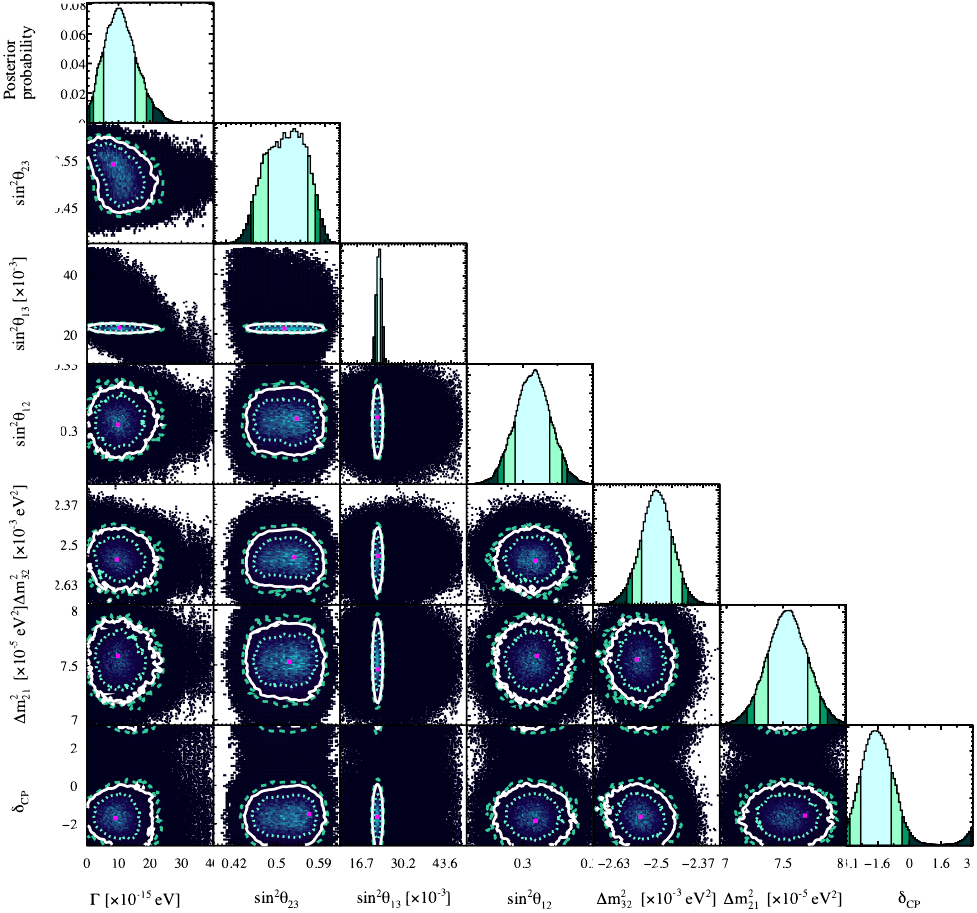
\includegraphics[width=1.\textwidth]{text/QD_asimov_wRC_trianglePlot_ih_screenshot.png}
	\caption{QD asimov wRC trianglePlot ih.}
	\label{fig:QD_asimov_wRC_trianglePlot_ih_screenshot}
    \end{figure}
%